\documentclass[../../report.tex]{subfiles}
\begin{document}
\section{Digital Music Representation}

So far, we have been using the terms \emph{music} and \emph{melody} rather
loosely. It is important that we clearly define the data format we will be
working with, as this directly influences the design of our neural network.

\subsection{Symbolic}

Much of the previous work in music generation has focused on the symbolic
domain. Generally, this includes any representation that abstracts away the
reproduction of sound, e.g. sheet music, chord progressions,
MIDI\footnote{Musical Instrument Digital Interface} events. This abstraction is
very appealing in the context of neural networks, as it greatly reduces the
amount of data to be processed, making the task more tractable. On the other
hand, this reduction comes at a cost. One cannot possibly hope to design a
symbolic encoding that captures the expression intricacies of every instrument,
let alone the complexity of vocals, therefore a loss in fidelity is inevitable.
\cite{Dieleman2020}

Given that this project is quite constrained in terms of computational
resources, we resort to modelling melodies in the symbolic domain. More
specifically, the training data shall be extracted from a large set of MIDI
files \todo{Data preparation section link}.

\subsubsection{MIDI}
MIDI is a technical standard introduced in 1983. It was designed to create a
universal interface for electronic music equipment, a market which was, at the
time, fragmented with incompatible standards.

MIDI devices communicate by means of a serial stream of bytes. A single MIDI
message consists of a status byte, generally followed by one or two data bytes.
There are many types of messages, but arguably the most important ones are
\emph{note-on} and \emph{note-off} events -- they represent the activation and
release of individual notes, effectively encoding a musical performance. Most
importantly, this sequence of events (figure \ref{fig:piano-roll}) can be saved
as a Standard MIDI File (SMF). Due to its popularity and portability, this
format is perfect for a sequence modelling application. \cite{MIDI2015Messages,
MIDI2015Files}

\begin{figure}
  \centering
  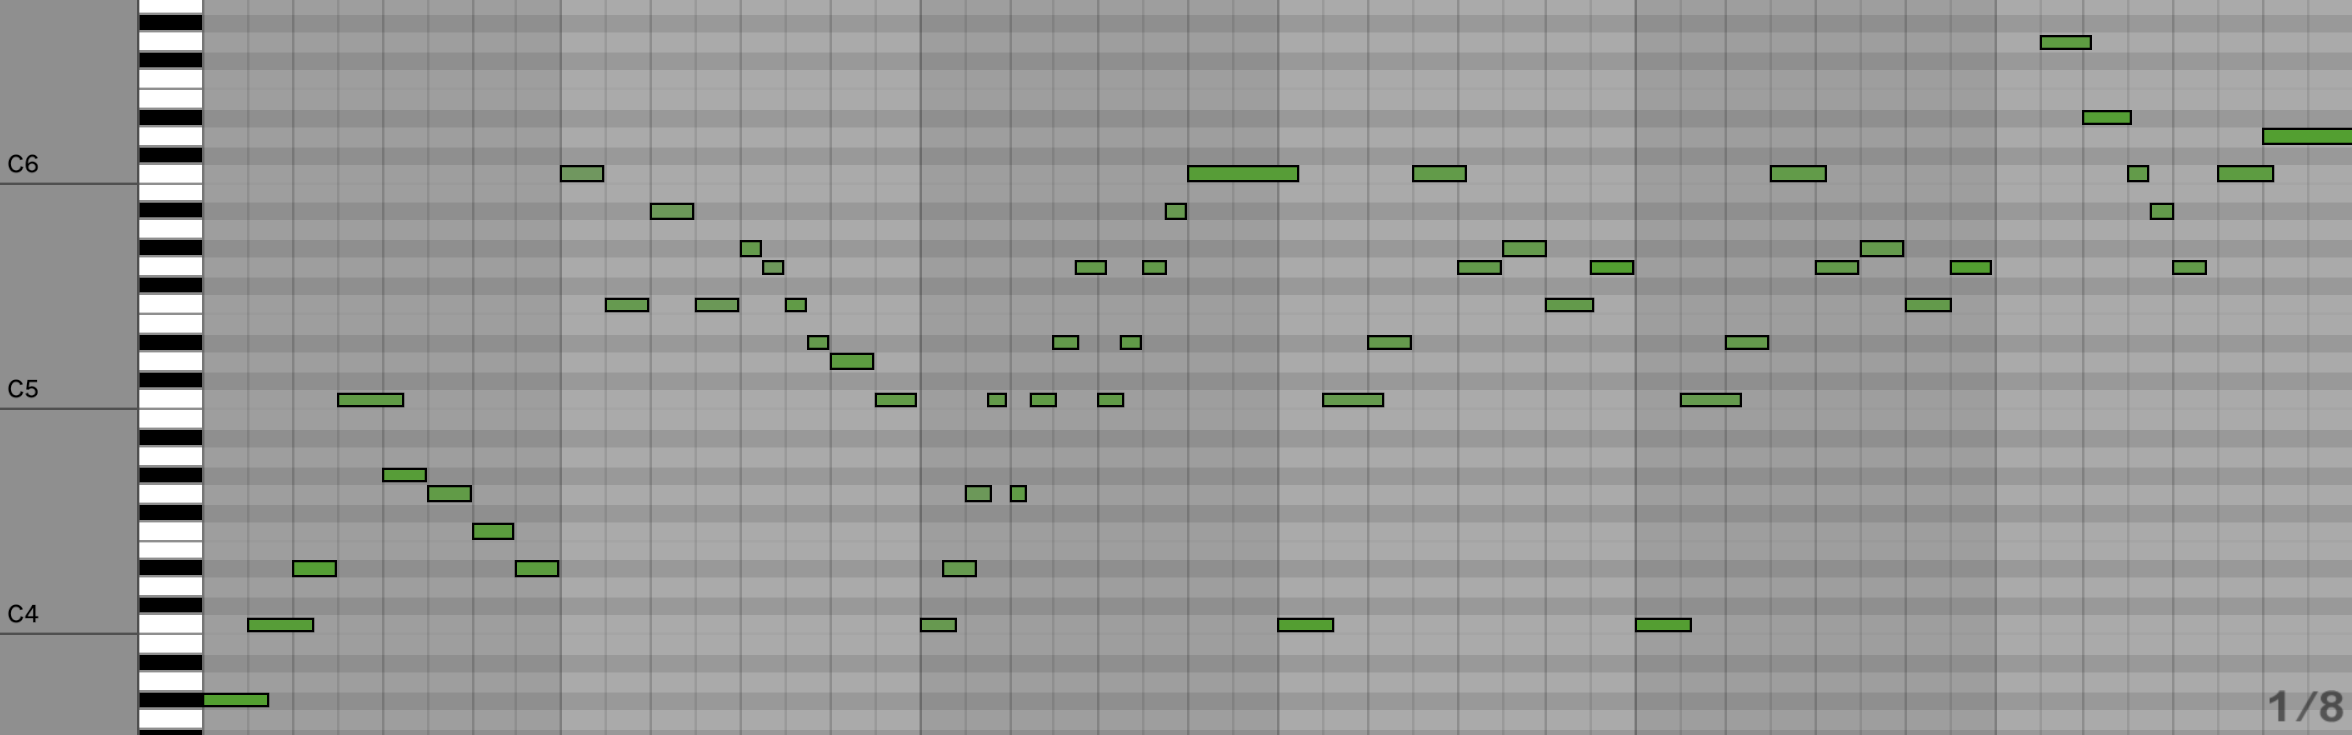
\includegraphics[width=\textwidth]{piano-roll}
  \caption{MIDI events in a digital audio workstation}
  \label{fig:piano-roll}
\end{figure}

\subsection{Waveform}

At the most fundamental level, music can be interpreted as an audio signal in
the time domain. Using pulse-code modulation (PCM), the otherwise continuous
signal is discretised in dimensions of both time and amplitude (figure
\ref{fig:pcm}). This produces a sequence of samples, which can then be fed into
a neural network. The benefit of this approach is that it inherently captures
intricate acoustic features, which may be lost in symbolic representations.
\cite{Dieleman2020}

Unfortunately, PCM produces immensely long sequences. Human hearing is limited
to frequencies below \num{20} kHz, and by the Nyquist--Shannon sampling theorem
we know that to capture all information in that range, the sampling frequency
must be at least twice that, i.e. \num{40} kHz or more. This means that one
second of audio is represented by \num{40000} steps, and usually generative
models are required to produce several seconds of audio. This can get out of
hand quickly, therefore many models have opted for a reduced sample rate of
\num{16} or \num{24} kHz, striking a balance between fidelity and computational
complexity. \cite{Dieleman2020}

\begin{figure}
  \centering
  \begin{subfigure}[b]{0.24\textwidth}
    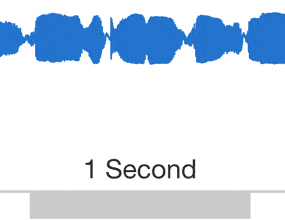
\includegraphics[width=\textwidth]{wave-1000ms}
  \end{subfigure}
  \hfill
  \begin{subfigure}[b]{0.24\textwidth}
    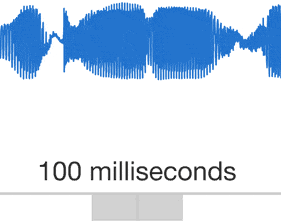
\includegraphics[width=\textwidth]{wave-100ms}
  \end{subfigure}
  \hfill
  \begin{subfigure}[b]{0.24\textwidth}
    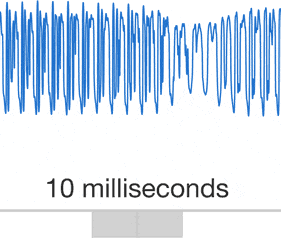
\includegraphics[width=\textwidth]{wave-10ms}
  \end{subfigure}
  \hfill
  \begin{subfigure}[b]{0.24\textwidth}
    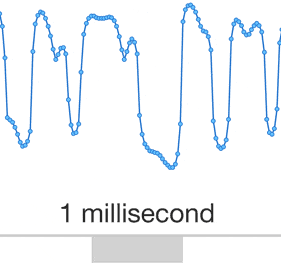
\includegraphics[width=\textwidth]{wave-1ms}
  \end{subfigure}
  \caption{PCM-encoded audio waveform \cite{Oord2016}}
  \label{fig:pcm}
\end{figure}

\subsection{Spectrum}

The same audio signal may also be represented in the frequency domain. By
applying the Fourier transform to a time-domain signal, one can obtain the
magnitude and phase of its frequency components at each point in time. Using
overlapping windows of several time-domain samples, the size of the sequences'
temporal dimension can be reduced considerably. However, in doing so, the amount
of information to be processed at each time step is increased. This means that a
frequency domain representation is not guaranteed to be more computationally
efficient. \cite{Dieleman2020}

Moreover, working in the frequency domain implies separating the magnitude and
phase components of a signal. While the magnitude exhibits reasonable
consistency, the phase is seemingly random (figure \ref{fig:spectrogram}). This
is a non-trivial hurdle for generative models, because the relative phase of a
signal's constituent frequencies encodes a great deal of perceptual details.
Solutions exist, but for now, time domain audio seems to be better suited for
generative models. \cite{Dieleman2020}

\begin{figure}
  \centering
  \begin{subfigure}[b]{0.49\textwidth}
    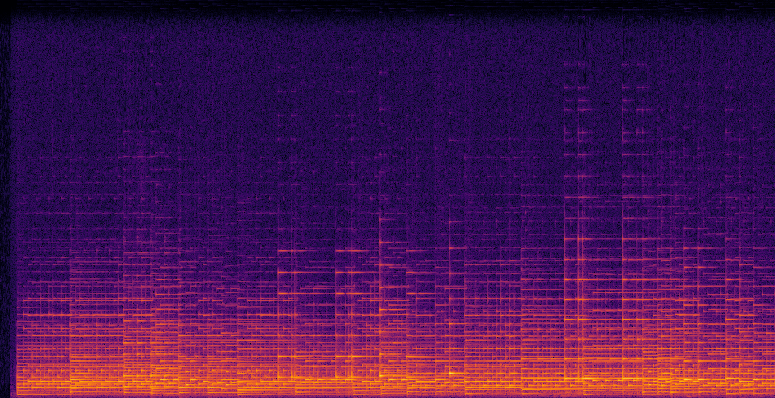
\includegraphics[width=\textwidth]{spectrogram-magnitude}
    \caption{Magnitude}
  \end{subfigure}
  \hfill
  \begin{subfigure}[b]{0.49\textwidth}
    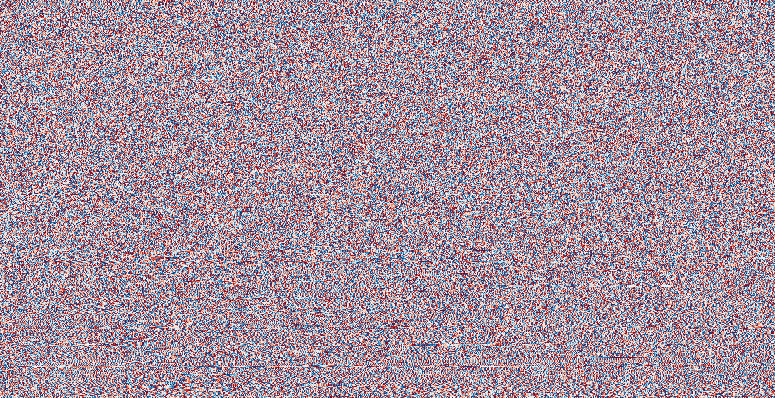
\includegraphics[width=\textwidth]{spectrogram-phase}
    \caption{Phase}
  \end{subfigure}
  \caption{Spectrogram of a piano recording \cite{Dieleman2020}}
  \label{fig:spectrogram}
\end{figure}

\end{document}
